\documentclass[10pt,a4paper]{article}

\usepackage{appendix}
\usepackage{graphicx}
\usepackage{parskip}
\usepackage{listings}
\usepackage{caption}
\usepackage{subcaption}
\usepackage{amsmath}
\usepackage{listings}
\usepackage{xcolor}
\usepackage[most]{tcolorbox}

%%%%%%%%%%%%%%%%%%%%%%%%%%%%%%%%%%%%%%%%%%%%%%%%%%%%%%%%%%%%%%%%%%%%%%%%%%%%%%%%%%%%%%%%%%%%%%%%%%%%%%%%%%
\definecolor{codegreen}{rgb}{0,0.6,0}
\definecolor{codegray}{rgb}{0.5,0.5,0.5}
\definecolor{codepurple}{rgb}{0.58,0,0.82}
\definecolor{backcolour}{rgb}{1,1,1}

\lstdefinestyle{mystyle}
{
    backgroundcolor=\color{backcolour},   
    commentstyle=\color{codegreen},
    keywordstyle=\color{magenta},
    numberstyle=\tiny\color{codegray},
    stringstyle=\color{codepurple},
    basicstyle=\ttfamily\footnotesize,
    breakatwhitespace=false,         
    breaklines=true,                 
    captionpos=b,                    
    keepspaces=true,                 
    numbers=left,                    
    numbersep=5pt,                  
    showspaces=false,                
    showstringspaces=false,
    showtabs=false,                  
    tabsize=2
}

\lstset{style=mystyle}
%%%%%%%%%%%%%%%%%%%%%%%%%%%%%%%%%%%%%%%%%%%%%%%%%%%%%%%%%%%%%%%%%%%%%%%%%%%%%%%%%%%%%%%%%%%%%%%%%%%%%%%%%%

\lstset{basicstyle=\ttfamily, breaklines = true, tabsize=2}
\graphicspath{ {./Images/} }
\setlength{\parskip}{1em}
\begin{document}
%%%%%%%%%%%%%%%%%%%%%%%%%%%%%%%%%%%%%%%%%%%%%%%%%%%%%%%%%%%%%%%%%%%%%%%%%%%%%%%%%%%%%%%%%%%%%%%%%%%%%%%%%%

\begin{titlepage}
	\centering
	{\scshape\LARGE Imperial College London \par}
	\vspace{1cm}
    {\scshape\Large ISA and Compilers: Year 2\par}
    \vspace{1.5cm}
	{\huge\bfseries ALU \par}
	\vspace{2cm}
	{\Large\ Xin Wang }
	\vfill
	{\large \today\par}
\end{titlepage}

%%%%%%%%%%%%%%%%%%%%%%%%%%%%%%%%%%%%%%%%%%%%%%%%%%%%%%%%%%%%%%%%%%%%%%%%%%%%%%%%%%%%%%%%%%%%%%%%%%%%%%%%%%

\begin{abstract}
    Unlike other instruction architectures like the Mu0, the ALU is used in almost every instruction
    in the MIPS architecture from common arithmetic to address calculation. 

    MIPS architecture supports negative and positive arithmetic as well as floating numbers i.e.
    decimals so it is important to understand how the ALU enables those features. Also the following
    aspects need to be studied:
    \begin{itemize}
        \item What about fractions and other real numbers?
        \item What happens if an operation creates a number bigger than can be represented?
        \item How  does  hardware  really multiply or divide numbers?
    \end{itemize}
\end{abstract}

%%%%%%%%%%%%%%%%%%%%%%%%%%%%%%%%%%%%%%%%%%%%%%%%%%%%%%%%%%%%%%%%%%%%%%%%%%%%%%%%%%%%%%%%%%%%%%%%%%%%%%%%%%

\tableofcontents
\pagebreak

%%%%%%%%%%%%%%%%%%%%%%%%%%%%%%%%%%%%%%%%%%%%%%%%%%%%%%%%%%%%%%%%%%%%%%%%%%%%%%%%%%%%%%%%%%%%%%%%%%%%%%%%%%
\section{Signed and unsigned numbers}

Numbers in computer hardware are represented as a series of high and low electronic signals i.e.
binary numbers. A single digit of a binary number is thus the “atom” of computing, since all 
information is composed of binary digits or bits. 

\begin{tcolorbox}[breakable,colback=white]
\textbf{Binary digit}: One of the two numbers in base 2 i.e. $0$ or $1$ that represents the components of information.
\end{tcolorbox}

\begin{figure} [h!]
    \centering
    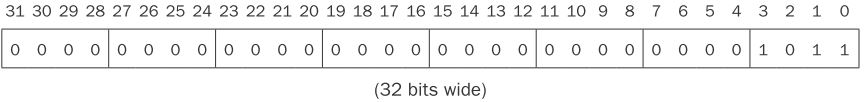
\includegraphics[scale=0.65]{MIPS 32 bit.JPG}
    \caption{Standard word length in MIPS architecture}
\end{figure}

The MIPS word is 32 bits long, so can represent $2^{32}$ different 32-bit patterns i.e. $0$ to $2^{32}-1$ 

\begin{tcolorbox}[breakable,colback=white]
\textbf{Least significant bit}: The \textbf{rightmost} bit in a MIPS word.
\\
\\
\textbf{Most significant bit}: The \textbf{leftmost} bit in a MIPS word.
\end{tcolorbox}

Hardware is designed to add, subtract, multiply, and divide these binary bit patterns. If the proper
result of such operations cannot be represented by these hardware bits, \textbf{overflow} has occurred. It’s up to the programming language, the operating system, and the program to determine what to do if overflow occurs.

Computer programs calculate both positive and negative numbers, so a system to distinguishes the
positive from the negative is needed:
\begin{enumerate}
    \item \textbf{Sign and magnitude}: Simplest system but adders for sign and magnitude will need
    an extra step to set the sign because it is not known in advance what the proper sign will be.
    Also, a separate sign bit means that sign and magnitude has both a positive and a negative 
    zero, which can lead to problems.
    \item \textbf{Two’s complement}: Leading $0$s mean positive, and leading $1$s mean negative. It
    has the advantage that all negative numbers have a $1$ in the most significant bit i.e. \textbf{the sign
    bit}. Hardware needs to test only the sign bit to see if a number is positive or negative. Overflow 
    can occur when the sign bit is incorrect e.g. a $0$ on the left of the bit pattern when the number is negative or a $1$ when the number is positive.
\end{enumerate}

\pagebreak

Two's complements are used in modern designs and there are two convenient shortcuts when dealing
with them:
\begin{enumerate}
    \item A quick way to negate a two’s complement binary number. 
    
    Invert every $0$ to $1$ and every 1 to 0, then add $1$ to the result. The reason is based on the
    observation that the sum of a number $x$ and its inverted $\overline{x}$ must be $-1$. Since
    $x+\overline{x}=-1$, the following statements are true:
    \begin{itemize}
        \item $x+\overline{x}+1=0$
        \item $\overline{x}+1=-x$
    \end{itemize}
    \item How to convert a binary number represented in $n$ bits e.g. $16$ bits to a number
    represented with \textbf{more than $n$ bits} e.g. $32$ bits. 

    \textbf{Sign extension}: Take the sign bit from the smaller quantity and copy it to fill the new
    bits of the larger quantity. This works because positive two’s complement numbers really have an
    infinite number of $0$s on the left and negative two’s complement numbers have an infinite
    number of $1$s. The binary bit pattern representing a number hides leading bits to fit the
    width of the hardware and sign extension simply restores some of them.
\end{enumerate}

%%%%%%%%%%%%%%%%%%%%%%%%%%%%%%%%%%%%%%%%%%%%%%%%%%%%%%%%%%%%%%%%%%%%%%%%%%%%%%%%%%%%%%%%%%%%%%%%%%%%%%%%%%
\section{Addition and Subtraction}

The simplest arithmetic operations. Digits are added bit by bit from right to left with carries
passed to the next digit to the left. Subtraction also uses the concept addition: the \textbf{operand is negated before being added}.

\begin{figure} [h!]
    \centering
    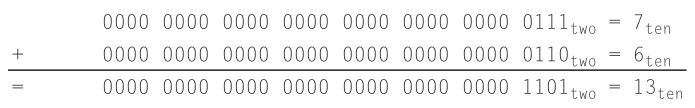
\includegraphics[scale=0.7]{Add.JPG}
    \caption{Addition: $7+6$}
\end{figure}

\begin{figure} [h!]
    \centering
    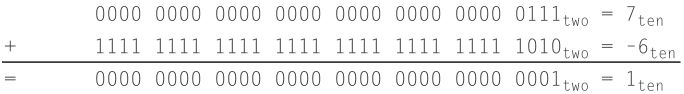
\includegraphics[scale=0.7]{Subtraction.JPG}
    \caption{Subtraction: $7-6$ where $6$ is in two's complement}
\end{figure}

A concern in any arithmetic operation is \textbf{overflow}. Recall that overflow occurs when the
result from an operation cannot be represented with the available hardware i.e. a $32$ bit word.  

Overflow can occur in \textbf{adding or subtracting two $32$-bit numbers with the same signs} which
yields a result that needs $33$ bits to be fully expressed. Overflow cannot occur when
\textbf{adding operands with different signs} because the sum is never larger than one of the
operands. 

\begin{tcolorbox}[breakable,colback=white]
    Overflows are easily detected by looking at the \textbf{sign bit}. Overflow occurs when adding two 
    positive numbers and the sum is negative, or vice versa. This means that a carry out occurred into the sign bit.
\end{tcolorbox}

\begin{figure} [h!]
    \centering
    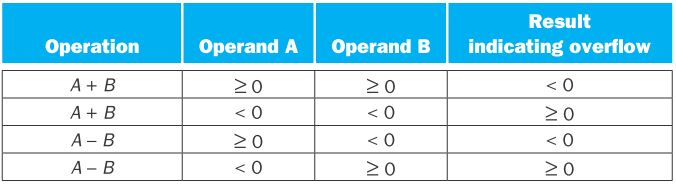
\includegraphics[scale=0.7]{Overflow.JPG}
    \caption{Overflow conditions for addition and subtraction}
\end{figure}

When dealing with \textbf{unsigned integers}, overflows are ignored as they are commonly used for
memory addresses and lack the sign bit. A computer architecture must therefore provide a way to
determine if overflow is important or not. 

The MIPS solution is to have two kinds of arithmetic instructions to recognize the two choices:
\begin{itemize}
    \item Add \texttt{add}, add immediate \texttt{addi} and subtract \texttt{sub} cause exceptions on 
    overflow.
    \item  Add unsigned \texttt{addu}, add immediate unsigned \texttt{addiu} and subtract unsigned \texttt{subu} do not cause exceptions on overflow.
\end{itemize}

\begin{tcolorbox}[breakable,colback=white]
\textbf{Interrupt}: An unscheduled event that disrupts program execution, commonly used to detect overflow.
\end{tcolorbox}

MIPS detects overflow with interrupts:
\begin{itemize}
    \item The address of the instruction that overflowed is saved in a register
    \item The computer jumps to a predefined address to invoke the appropriate routine for that 
    exception.
    \item The interrupted address is saved so that in some situations the program 
    can continue after corrective code is executed.
\end{itemize}  

\pagebreak

%%%%%%%%%%%%%%%%%%%%%%%%%%%%%%%%%%%%%%%%%%%%%%%%%%%%%%%%%%%%%%%%%%%%%%%%%%%%%%%%%%%%%%%%%%%%%%%%%%%%%%%%%%
\section{Multiplication}

First, a recap of the multiplication of decimal numbers by hand to establish the steps of
multiplication and the names of the operands. 

The following working example $1000_{ten}$ and $1001_{ten}$:
\begin{figure} [h!]
    \centering
    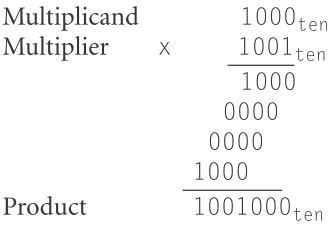
\includegraphics[scale=0.6]{Multiplication.JPG}
\end{figure}

There are two observations in the multiplication process:
\begin{itemize}
    \item The number of digits in the product is larger than the number in either the multiplicand
    or the multiplier. 
    
    The length of the multiplication of an $n$-bit multiplicand and an $m$-bit multiplier is a
    product that is $n+m$-bits long. That is, $n+m$-bits are required to represent all possible
    products.  Like add, multiplication must cope with overflow.
    \item Due to the binary design, there are only two possible actions at each step of multiplication:
    \begin{enumerate}
        \item Place a copy of the multiplicand i.e. $1 \times multiplicand$ in the proper place if
        \textbf{multiplier digit} is a $1$.
        \item Place $0$s i.e. $0 \times multiplicand$ in the proper place if \textbf{multiplier digit}
        is a $0$.
    \end{enumerate}
\end{itemize}

\pagebreak

%%%%%%%%%%%%%%%%%%%%%%%%%%%%%%%%%%%%%%%%%%%%%%%%%%%%%%%%%%%%%%%%%%%%%%%%%%%%%%%%%%%%%%%%%%%%%%%%%%%%%%%%%%
\subsection{Sequential version of the multiplication algorithm and Hardware}

Building, from the observations above, a simple design that supports only multiplying positive
numbers: \par
\begin{figure} [h!]
    \centering
    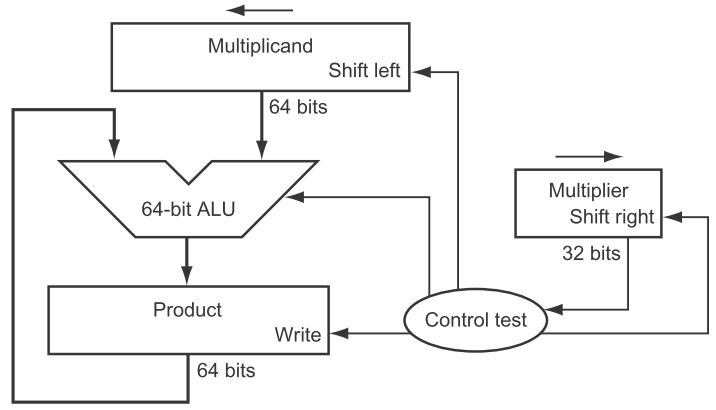
\includegraphics[scale=0.55]{Multiply path.JPG}
    \caption{First version of the multiplication hardware}
\end{figure}

\begin{figure} [h!]
    \centering
    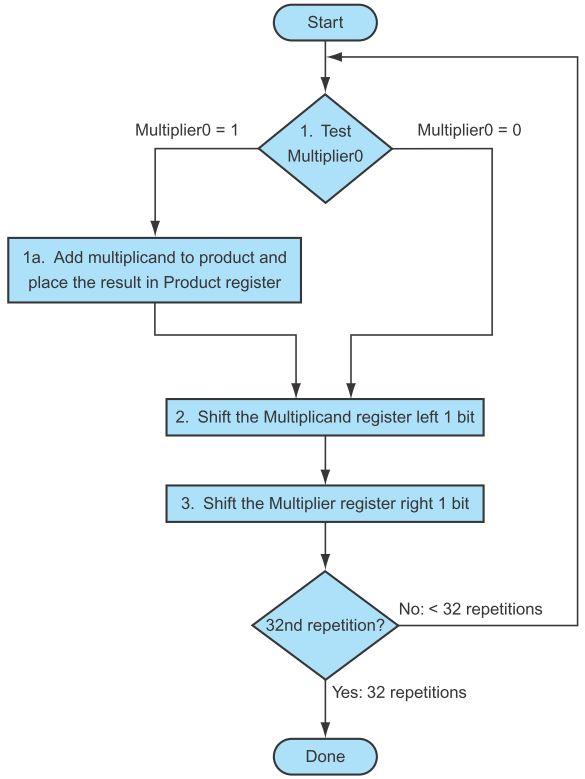
\includegraphics[scale=0.71]{Multiply flow.JPG}
    \caption{The first multiplication algorithm}
\end{figure}

Multiplication:
\begin{itemize}
    \item The multiplier is in the $32$-bit \textit{multiplicand register} and that the $64$-bit \textit{product register} is initialized to $0$. 
    \item From the example above, multiplying means moving the multiplicand left one digit each step
    since it may be added to the intermediate products. So that means over $32$ steps, a $32$-bit
    multiplicand would move $32$ bits to the left.
    \item  Hence, a 64-bit \textit{multiplicand register} is needed, initialized with the $32$-bit
    multiplicand \textbf{in the right half and zero in the left half}.
    \item The \textit{multiplicand register} is then shifted left $1$ bit each step to align the
    multiplicand with the sum being accumulated in the $64$-bit \textit{product register}.
    \item Control decides when to shift the \textit{Multiplicand register} and \textit{Multiplier register} and when to write new values into the Product register.
\end{itemize}   

\begin{figure} [h!]
    \centering
    \includegraphics[scale=0.75]{Multiply Example.JPG}
\end{figure}

Three steps of the flowchart:
\begin{itemize}
    \item  The least significant bit of the multiplier i.e. \textbf{Multiplier0} determines whether the multiplicand is added to the \textit{product register}.
    \item The left shift in step 2 has the effect of moving the intermediate operands to the left.
    \item The shift right in step 3 gives us the next bit of the multiplier to examine in the following iteration.
\end{itemize}

This simple algorithm would take more than one clock cycle. However, it can be easily refined to
take $1$ clock cycle per step by performing the operations in parallel i.e. the \textit{multiplier}
and \textit{multiplicand} are shifted while the \textit{multiplicand} is added to the product if the
multiplier bit is a 1.

The hardware has to ensure that it tests the right bit of the multiplier and gets the pre-shifted
version of the multiplicand.
\begin{figure} [h!]
    \centering
    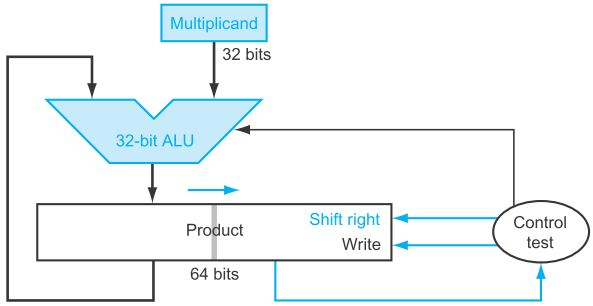
\includegraphics[scale=0.7]{Multiply path 2.JPG}
    \caption{Optimised version of the multiplication hardware}
\end{figure}

%%%%%%%%%%%%%%%%%%%%%%%%%%%%%%%%%%%%%%%%%%%%%%%%%%%%%%%%%%%%%%%%%%%%%%%%%%%%%%%%%%%%%%%%%%%%%%%%%%%%%%%%%%
\subsection{Signed multiplication}

Dealing with signs in multiplication is a simple addition on the existing system. The easiest way to
understand how to deal with signed numbers is:
\begin{itemize}
    \item Convert the \textit{multiplier} and \textit{multiplicand} to positive numbers.
    \item Remember the original signs
\end{itemize}  

The algorithms would then be run for 31 iterations as normally design, leaving the signs out of the
calculation. The shifting steps would need to extend the sign of the product for signed numbers.
When the algorithm completes, the lower word would have the 32-bit product.

%%%%%%%%%%%%%%%%%%%%%%%%%%%%%%%%%%%%%%%%%%%%%%%%%%%%%%%%%%%%%%%%%%%%%%%%%%%%%%%%%%%%%%%%%%%%%%%%%%%%%%%%%%
\subsection{Multiply in MIPS}

MIPS provides a separate pair of $32$-bit registers to contain the $64$-bit product called $Hi$ and
$Lo$. To produce proper signed or unsigned product, MIPS has two instructions: 
\begin{itemize}
    \item Multiply \texttt{mult}
    \item Multiply unsigned \texttt{multu}
\end{itemize} 

To fetch the integer $32$-bit product, the programmer uses instruction "move from lo" \texttt{mflo}.
The MIPS assembler generates a pseudoinstruction for multiply that specifies three general-purpose
registers, generating \texttt{mflo} and \texttt{mfhi} instructions to place the product into registers.

\pagebreak

%%%%%%%%%%%%%%%%%%%%%%%%%%%%%%%%%%%%%%%%%%%%%%%%%%%%%%%%%%%%%%%%%%%%%%%%%%%%%%%%%%%%%%%%%%%%%%%%%%%%%%%%%%
\section{Division}

The reciprocal of multiply that is less frequent and more complicated especially considering the opportunity to perform a mathematically invalid operation: dividing by 0.

Like multiplication, the classic pen-and-paper is first revised to establish some observations.

The example is dividing $1 001 010$ by $1000$: \par
\begin{figure} [h!]
    \centering
    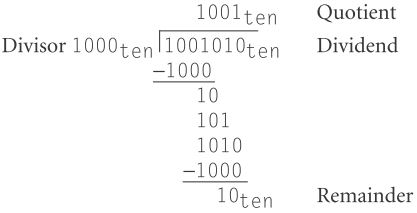
\includegraphics[scale=0.7]{Long division.JPG}
\end{figure}
There are:
\begin{itemize}
    \item \textbf{Two operands: Divisor and Dividend}
    \item \textbf{Two outputs: Quotient and Remainder}
\end{itemize}  
\begin{align*}
    \text{Dividend} = \text{Quotient} \times \text{Divisor} + \text{Remainder}
\end{align*}

%%%%%%%%%%%%%%%%%%%%%%%%%%%%%%%%%%%%%%%%%%%%%%%%%%%%%%%%%%%%%%%%%%%%%%%%%%%%%%%%%%%%%%%%%%%%%%%%%%%%%%%%%%
\subsection{Division algorithm and Hardware}

Start with the $32$-bit \textit{Quotient register} set to $0$. Each iteration of the algorithm needs
to \textbf{move the divisor to the right one digit}, so the \textbf{text} divisor placed in the left-half 
of the $64$-bit \textit{Divisor register} and shift it right 1 bit each step to align it with the 
dividend. The Remainder register is initialized with the dividend.
\begin{figure} [h!]
    \centering
    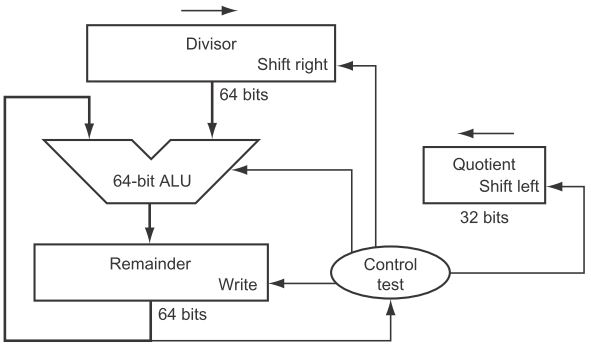
\includegraphics[scale=0.7]{Division.JPG}
    \caption{First version of the division hardware.}
\end{figure}

There are three steps of the division algorithm:
\begin{enumerate}
    \item The computer needs to know in advance if the divisor is smaller than the dividend. It
    subtracts the divisor since this is how comparisons are performed in the set on less than instruction.
    \begin{itemize}
        \item If result is positive, divisor is smaller or equal to the dividend. A $1$ is outputted in 
        the quotient.
        \item If result is negative, restore the original value by adding the divisor back to the
        remainder and output a $0$ in the quotient.
    \end{itemize}
    \item The divisor is shifted right and then repeated again.
    \item The remainder and quotient will be found in their respective registers after the iterations are complete.
\end{enumerate}     
\begin{figure} [h!]
    \centering
    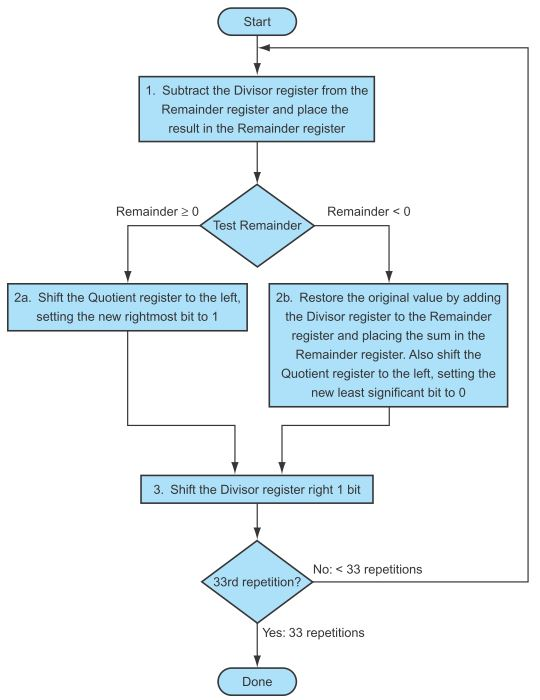
\includegraphics[scale=0.8]{Division flow.JPG}
\end{figure}
This algorithm and hardware can be refined to be faster and cheaper. The optimisation comes from
shifting the operands and the quotient \textbf{simultaneously with the subtraction}. This halves the
width of the adder and registers by noticing where there are unused portions of registers and
adders. 

\begin{figure} [h!]
    \centering
    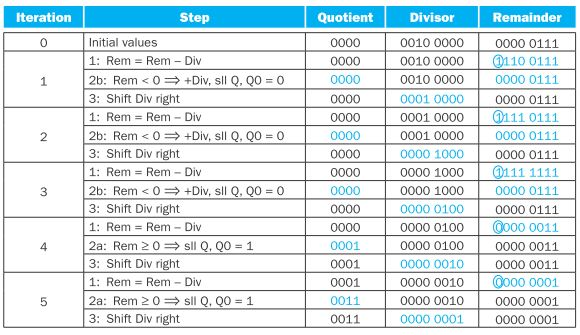
\includegraphics[scale=0.8]{Divide example.JPG}
\end{figure}

\begin{figure} [h!]
    \centering
    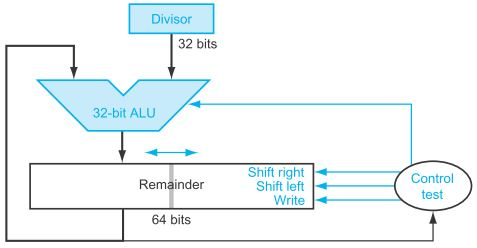
\includegraphics[scale=0.7]{Refined divide.JPG}
    \caption{An improved version of the division hardware}
\end{figure}

%%%%%%%%%%%%%%%%%%%%%%%%%%%%%%%%%%%%%%%%%%%%%%%%%%%%%%%%%%%%%%%%%%%%%%%%%%%%%%%%%%%%%%%%%%%%%%%%%%%%%%%%%%
\subsection{Signed division}

The simplest solution is to remember the signs of the divisor and dividend and then negate the
quotient if the signs disagree. Remember that the following equation must always hold:
\begin{align*}
    \text{Dividend} = \text{Quotient} \times \text{Divisor} + \text{Remainder}
\end{align*}

For example divide all the combinations of $(\pm) 7$ by $(\pm) 2$:
\begin{itemize}
    \item $(+)7 \div (+)2$: $\text{Quotient} = (+)3 \text{ and } \text{Remainder} = (+)1$
    \item $(-)7 \div (+)2$: $\text{Quotient} = (-)3 \text{ and } \text{Remainder} = (-)1$
    \item $(+)7 \div (-)2$: $\text{Quotient} = (-)3 \text{ and } \text{Remainder} = (+)1$
    \item $(-)7 \div (-)2$: $\text{Quotient} = (+)3 \text{ and } \text{Remainder} = (-)1$
\end{itemize}

The rule observed is that the dividend and remainder \textbf{must have the same signs}. The
correctly signed division algorithm:
\begin{itemize}
    \item Negates the quotient if the signs of the operands are opposite
    \item Makes the sign of the nonzero remainder match the dividend
\end{itemize} 

%%%%%%%%%%%%%%%%%%%%%%%%%%%%%%%%%%%%%%%%%%%%%%%%%%%%%%%%%%%%%%%%%%%%%%%%%%%%%%%%%%%%%%%%%%%%%%%%%%%%%%%%%%
\subsection{Divide in MIPS}

The same sequential hardware can be used for both multiply and divide. The only requirement is:
\begin{itemize}
    \item $64$-bit register that can shift left or right
    \item $32$-bit \textit{ALU}that adds or subtracts
\end{itemize}

Hence, MIPS uses the $32$-bit \texttt{Hi} and $32$-bit \texttt{Lo} registers for both multiply and divide.
\texttt{Hi} contains the remainder and \texttt{Lo} contains the quotient after the divide
instruction completes.

To handle both signed integers and unsigned integers, MIPS has two instructions: divide \texttt{div}
and divide unsigned \texttt{divu}.  

The MIPS assembler allows divide instructions to specify three registers, generating the
\texttt{mflo} or \texttt{mfhi} instructions to place the desired result into a general-purpose register.

\pagebreak

%%%%%%%%%%%%%%%%%%%%%%%%%%%%%%%%%%%%%%%%%%%%%%%%%%%%%%%%%%%%%%%%%%%%%%%%%%%%%%%%%%%%%%%%%%%%%%%%%%%%%%%%%%
\section{Constructing a basic ALU}

The \textit{ALU} is the brain of the computer, the device that performs the
arithmetic operations like addition and subtraction or logical operations like AND and OR. Because
the MIPS word is 32 bits wide, a 32-bit-wide \textit{ALU} is needed.

%%%%%%%%%%%%%%%%%%%%%%%%%%%%%%%%%%%%%%%%%%%%%%%%%%%%%%%%%%%%%%%%%%%%%%%%%%%%%%%%%%%%%%%%%%%%%%%%%%%%%%%%%%
\subsection{1-bit ALU}

The logical operations are easiest, because they map directly onto the hardware components. 
\begin{figure} [h!]
    \centering
    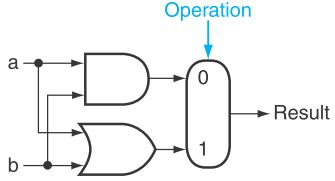
\includegraphics[scale=0.7]{1 bit ALU.JPG}
    \caption{1-bit logical unit for AND and OR}
\end{figure}

The multiplexor on the right then selects $a$ AND $b$ or $a$ OR $b$, depending on whether the value 
of Operation is 0 or 1.

The next function to include is addition:
\begin{itemize}
    \item An adder must have \textbf{two inputs} for the operands and a \textbf{single-bit output} for the sum.
    \item There must be a second output to pass on the carry \texttt{CarryOut}.
    \item Since the \texttt{CarryOut} from the neighbor adder must be included as an input, a third
    input \texttt{CarryIn} is defined.
\end{itemize}  

\begin{figure} [h!]
    \centering
    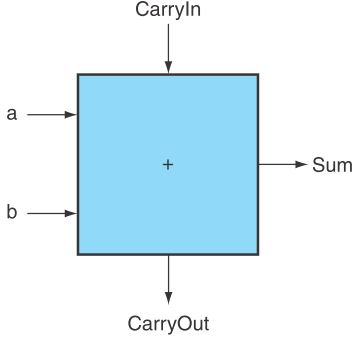
\includegraphics[scale=0.6]{Adder.JPG}
    \caption{A 1-bit adder}
\end{figure}

\pagebreak

The output functions \texttt{CarryOut} and \texttt{Sum} can be defined as logical equations and
implemented with logic gates.
\begin{figure} [h!]
    \centering
    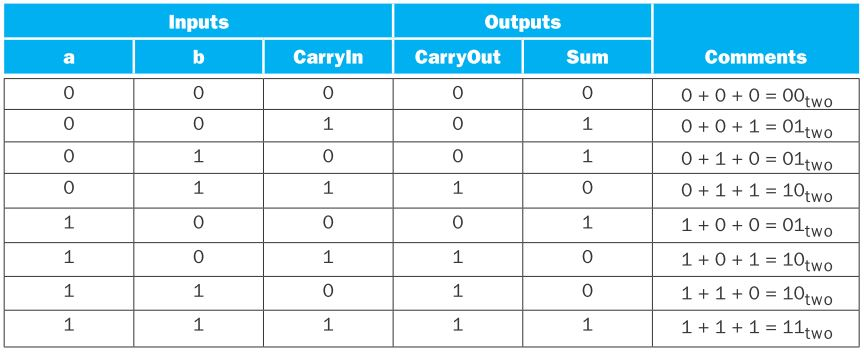
\includegraphics[scale=0.7]{Adder table.JPG}
    \caption{Input and output specification for a 1-bit adder.}
\end{figure}

1-bit ALU derived by combining the adder with the earlier components. If designers want the ALU to
perform a few more simple operations such as generating 0, the easiest way to add an operation is to 
expand the multiplexor controlled by the Operation line.
\begin{figure} [h!]
    \centering
    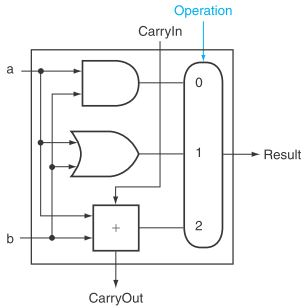
\includegraphics[scale=0.8]{ALU.JPG}
    \caption{A 1-bit ALU that performs AND, OR, and addition}
\end{figure}

\pagebreak

%%%%%%%%%%%%%%%%%%%%%%%%%%%%%%%%%%%%%%%%%%%%%%%%%%%%%%%%%%%%%%%%%%%%%%%%%%%%%%%%%%%%%%%%%%%%%%%%%%%%%%%%%%
\subsection{32-bit ALU}

The full $32$-bit ALU is created by connecting adjacent $1$-bit ALUs. The adder created by directly
linking the carries of 1-bit adders is a \textbf{ripple carry adder}.
\begin{figure} [h!]
    \centering
    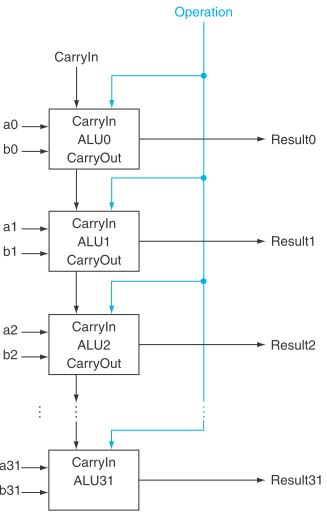
\includegraphics[scale=0.7]{32 ALU.JPG}
    \caption{A 32-bit ALU constructed from 32 1-bit ALUs}
\end{figure}

Remember, subtraction is the same as adding the negative version of an operand and this is how
adders would perform subtraction. The shortcut for negating a two’s complement number is to invert
each bit and then add 1. 

To invert each bit, add a $[2:1]$ multiplexor that chooses between $b$ and $\overline{b}$ \par
\begin{figure} [h!]
    \centering
    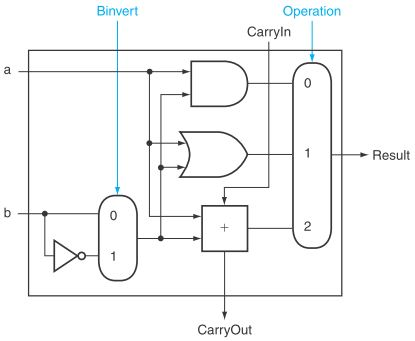
\includegraphics[scale=0.7]{ALU subtract.JPG}
    \caption{A 1-bit ALU that performs AND, OR, and addition on $a$ and $b$ or $a$ and $\overline{b}$}
\end{figure}

\pagebreak

The simplicity of the hardware design of a two’s complement adder helps explain why two’s complement
representation has become the universal standard for integer computer arithmetic.

%%%%%%%%%%%%%%%%%%%%%%%%%%%%%%%%%%%%%%%%%%%%%%%%%%%%%%%%%%%%%%%%%%%%%%%%%%%%%%%%%%%%%%%%%%%%%%%%%%%%%%%%%%
\subsection{Tailoring the 32-Bit ALU to MIPS}

The previous section implemented $add$, $sub$, $AND$ and $OR$. There is one last instruction that is
performed by the \textit{ALU} in the MIPS architecture: "set on less than" \texttt{slt}.

The \texttt{slt} instruction sets the destination register's content to the value $1$ if the first source
register's contents are less than the second source register's contents i.e. $rs < rt$. Otherwise, it is set to the
value 0.
\begin{align*}
    slt \; \$\text{destination}, \: \$ \text{first source address}, \: \$\text{second source address}
\end{align*}

To add support for this instruction, the ALU needs to expand the three-input multi-plexor to add an input for the \texttt{slt} result. 
\begin{figure} [h!]
    \centering
    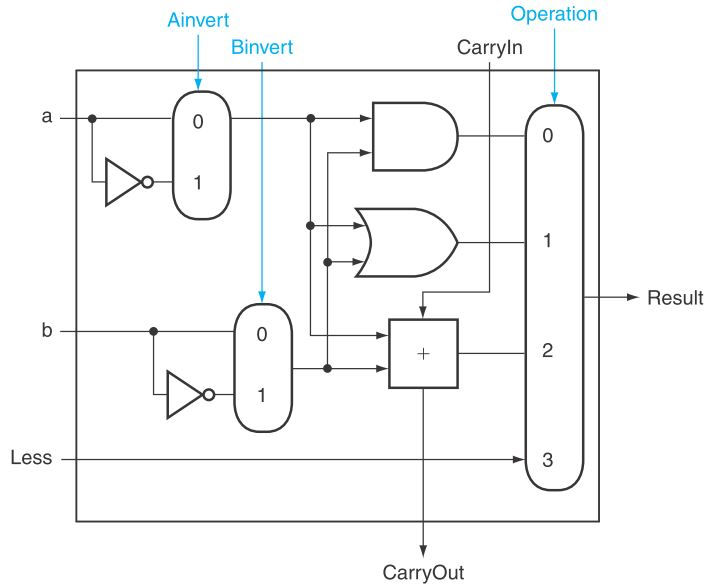
\includegraphics[scale=0.6]{slt.JPG}
\end{figure}

From the description of \texttt{slt}, the upper $31$ bits of the \textit{ALU} are always $0$. What
remains to consider is how to compare and set the least significant bit for "set on less than"
instructions.

Note that subtraction can be used, if the difference is negative then $a < b$:
\begin{align*}
    (a-b) < 0 &\Rightarrow ((a-b)+b)<(0+b) \\
    &\Rightarrow a<b
\end{align*} 
A $1$ if $a < b$ is negative and a $0$ if it’s positive. This result corresponds exactly to the sign
bit values. Following this line of argument, just connect the sign bit from the adder output.

Some modifications to the existing \textit{ALU} is required to support the \texttt{slt} instruction.

\begin{figure} [h!]
    \centering
    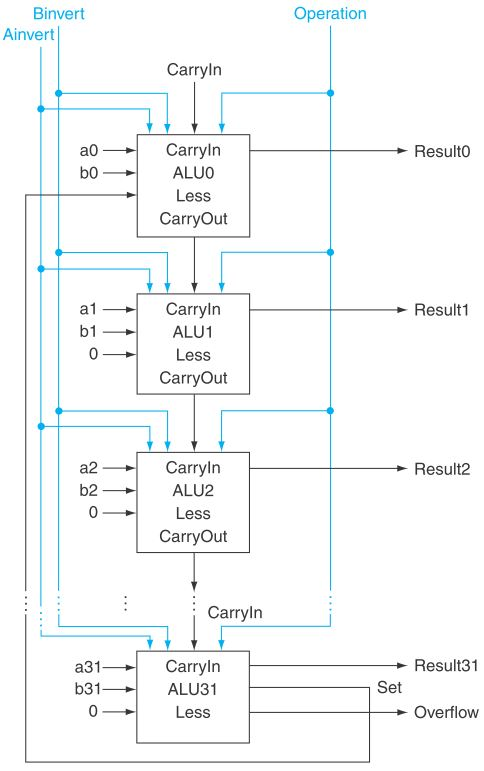
\includegraphics[scale=0.7]{ALU 2.JPG}
    \caption{ A 32-bit ALU constructed from the 31 copies of the 1-bit ALU as seen previously and one 1-bit ALU in the bottom.}
\end{figure}

The \texttt{Less} inputs are connected to $0$ except for the least significant bit, which is
connected to the \texttt{Set} output of the most significant bit:
\begin{itemize}
    \item If the \textit{ALU} performs $a - b$, the input 3 in the multiplexor shows \texttt{Result}$=0\dots 001$
    \item If the \textit{ALU} performs $a < b$, the input 3 in the multiplexor shows \texttt{Result}$=0\dots 000$
\end{itemize} 

\pagebreak

%%%%%%%%%%%%%%%%%%%%%%%%%%%%%%%%%%%%%%%%%%%%%%%%%%%%%%%%%%%%%%%%%%%%%%%%%%%%%%%%%%%%%%%%%%%%%%%%%%%%%%%%%%
\section{MIPS in Verilog}

\begin{figure} [h!]
    \centering
    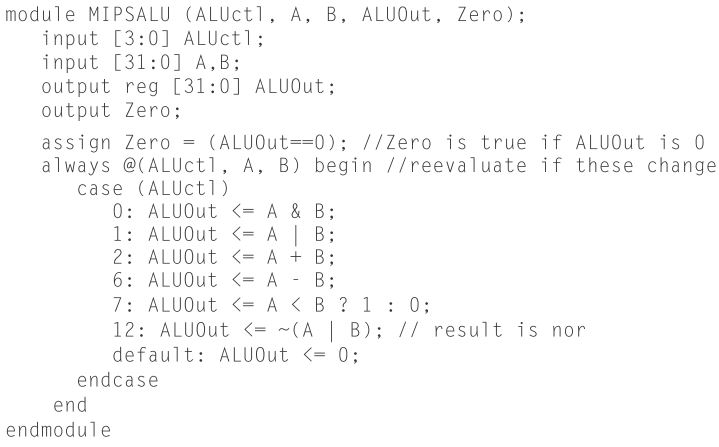
\includegraphics[scale=0.7]{ALU verilog.JPG}
    \caption{Verilog behavioral definition of a MIPS ALU.}
\end{figure}

\begin{figure} [h!]
    \centering
    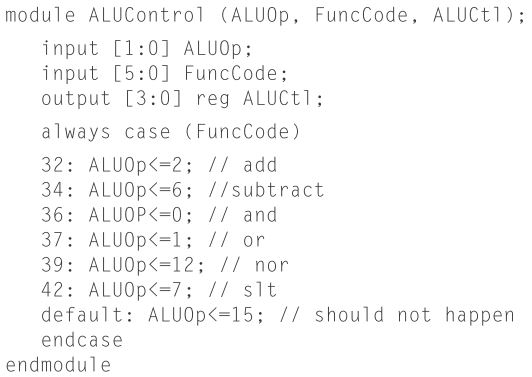
\includegraphics[scale=0.7]{ALU control verilog.JPG}
    \caption{MIPS ALU control: Combinational control logic.}
\end{figure}


%%%%%%%%%%%%%%%%%%%%%%%%%%%%%%%%%%%%%%%%%%%%%%%%%%%%%%%%%%%%%%%%%%%%%%%%%%%%%%%%%%%%%%%%%%%%%%%%%%%%%%%%%%
\end{document}